\documentclass[oneside]{beamer}


%*****************************************************************************%
%   Theme para la Presentación                                                %
%*****************************************************************************%
\usetheme[pageofpages=de,% String used between the current page and thetotal page count.
          bullet=circle,% Use circles instead of squares for bullets.
          titleline=true,% Show a line below the frame title.
          alternativetitlepage=true,% Use the fancy title page.
          titlepagelogo=../book/graphics/logo.png,% Logo for the first page.
          ]{Torino}
% Nouvelle is a green and red alternative to the chameleon color theme.
\usecolortheme{freewilly}
\providecommand*{\eqcolon}{\mathrel{=\!\raise.16ex\hbox{\footnotesize\!:}}} % para las definiciones

%*****************************************************************************%
%   Paquetes principales                                                      %
%*****************************************************************************%
\usepackage{amssymb, amsmath}
\usepackage{amsthm}
\usepackage{amsfonts}
\usepackage{float}
\usepackage{afterpage}
\usepackage{dsfont}
\usepackage{url}
\usepackage{color}
\usepackage{lettrine}
\usepackage{algorithm}
\usepackage{algpseudocode}
\usepackage{graphicx}
%\usepackage{subfig}
\usepackage{caption}
\usepackage{subcaption}
\usepackage{multimedia}
\usepackage{verbatim} % comentarios
\usepackage{pdfpages}
\usepackage[spanish]{babel}
\usepackage[utf8]{inputenc}
\usepackage{textcomp}

%Para determinar la fecha actual
\newcommand{\monthname}{\ifcase\month\or Enero\or Febrero\or
      Marzo\or Abril\or Mayo\or Junio\or Julio\or Agosto\or Septiembre\or
      Octubre\or Noviembre\or Diciembre\fi}

\newcommand{\thismonth}{\monthname,\ \the\year}


\author{\  \\ Maximiliano Báez González}
\title{Modelo predictivo de focos de dengue aplicado a Sistemas de Información Geográfica}
\institute{Facultad Politécnica- UNA}
%pone la fecha de generación como portada
\date{\thismonth}


\begin{document}
\renewcommand{\inserttotalframenumber}{54}
\begin{frame}[t,plain]
\titlepage
\end{frame}
%----------------------------1----------------------------------
\begin{frame}[t]{Motivación y Definición del Problema.}
  \begin{center}
    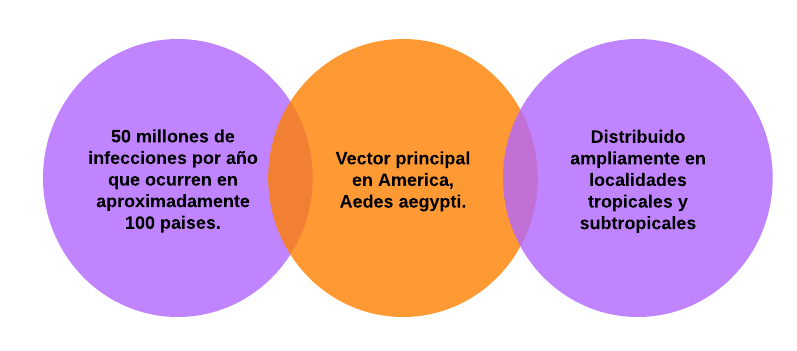
\includegraphics[width=10cm]{./graphics/dengue-intro.png}
  \end{center}
\end{frame}

%----------------------------2----------------------------------

\begin{frame}[t]{Motivación y Definición del Problema.\\\textit{Criaderos del Aedes aegypti.}}
\begin{center}
    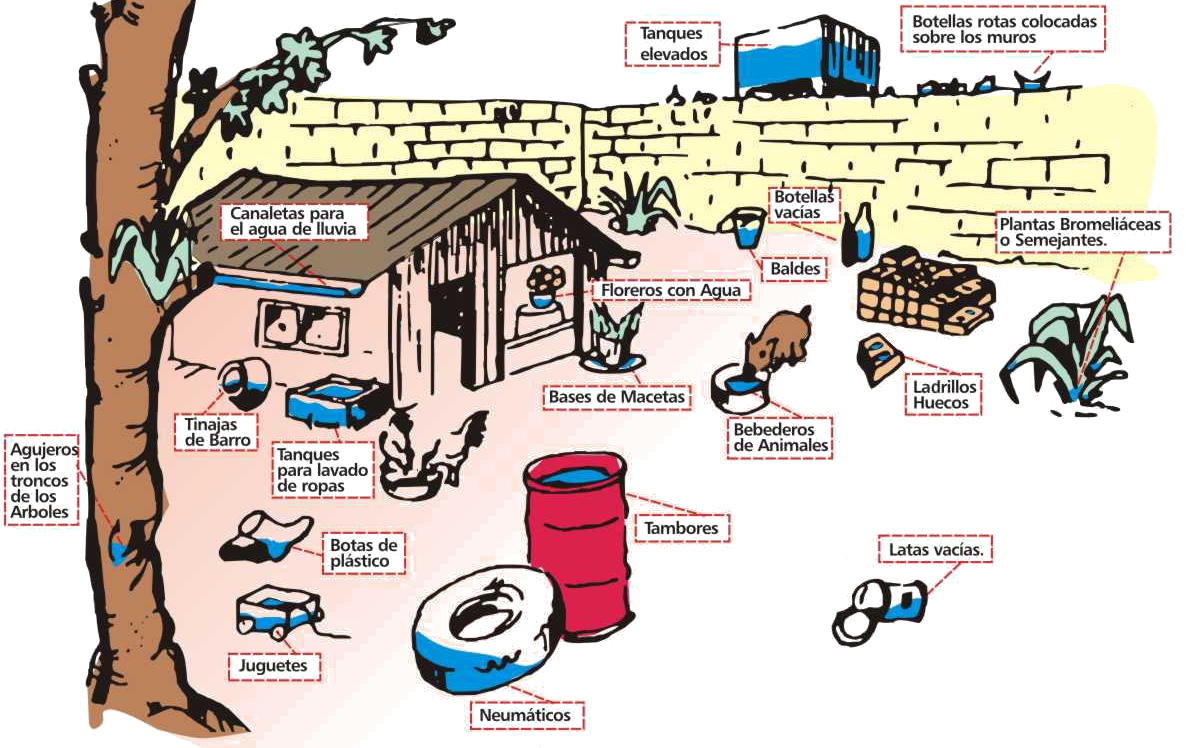
\includegraphics[width=9cm]{./graphics/criaderos.jpg}
    \end{center}
\end{frame}

%----------------------------3----------------------------------


%----------------------------4----------------------------------

\begin{frame}[t]{Motivación y Definición del Problema.\\\textit{Dengue en Paraguay.}}
  \begin{center}
    \begin{itemize}
    \item El Paraguay desde el año 2009 es considerado un país endémico.

    \item El clima, subtropical, favorece la aparición y desarrollo del dengue.

    \item Se realizan actividades de monitoreo del comportamiento el vector mediante técnicas tradicionales de vigilancia.

    \item Se utilizan técnicas de control vectorial, como fumigación, para la disminución de las poblaciones de mosquitos.

    \item En las últimas décadas se han observado un crecimiento considerable de las notificaciones de posibles casos de dengue, algunas con derivaciones fatales.
    \end{itemize}
  \end{center}
\end{frame}

%----------------------------5----------------------------------

\begin{frame}[t]{Motivación y Definición del Problema.\\\textit{Dengue en Paraguay.}}
  \begin{center}
  \begin{table}
      \begin{minipage}{\textwidth}
          \begin{center}
          \caption{Histórico de casos de dengue notificados, confirmados y con derivación fatal en Paraguay.}
          \begin{tabular}{l c c r r}
              \hline
              Año & Periodo (inicio / fin) & Notificados & Confirmados & Muertes\\
              \hline
              \hline
              2014 & 29-12-13 / 31-05-14 & 10.541 & 1.052 & 2\\
              2013 & 30-12-12 / 21-12-13 & 153.793 & 131.306 & 70\\
              2012 & 01-01-12 / 22-12-12 & 37.815 & 30.588 & 11\\
              2011 & 03-01-11 / 29-12-11 & 53.397 & 42.264 & 62\\
              2010 & 11-10-09 / 25-12-10 & 21.951 & 13.760 & --$^a$
          \end{tabular}
          \footnotetext[1]{No se encontraron datos sobre muertes en el periodo.}
          \end{center}
      \end{minipage}
  \end{table}
  \end{center}
\end{frame}

%----------------------------6----------------------------------

\begin{frame}[c]{Motivación y Definición del Problema.\\\textit{Vigilancia Entomológica en Paraguay.}}

    \begin{itemize}
      \item La Vigilancia Entomológica es un proceso orientado al levantamiento de información sobre la distribución del vector.

      \item Para estimar la densidad del vector, la OMS ha recomendado los siguientes indicadores entomológicos : Índice de Casa, Índice de Recipiente e Índice de Breteau.

      \item Sólo son recomendados para detectar la calidad de las acciones realizadas por el personal de control larvario.

      \item Las autoriadades sanitarias del Paraguay utilizan estos índices para estimar la densidad poblacionál del vector.

    \end{itemize}
\end{frame}

\begin{frame}[c]{Motivación y Definición del Problema.\\\textit{Vigilancia Entomológica en Paraguay.}}
\begin{itemize}
      \item Actualmente son considerados, por la OMS, como una pobre indicación de la producción de mosquitos adultos.

      \item No reflejan la asociación que existe entre las densidades de mosquitos y los tipos de recipientes.

      \item Proporcionan poca o nula información de aquellas viviendas en las que existe un mayor riesgo de presencia de mosquitos.

      \item Existen numerosos métodos e indicadores más prácticos, eficientes y económicos, como larvitrampas y ovitrampas\footnote{Centro Nacional de Programas Preventivos y Control de Enfermedades. \textit{Guía para la Vigilancia Entomológica con Ovitrampas}. Oct 2013.\\}.

    \end{itemize}
\end{frame}

%----------------------------7----------------------------------

\begin{frame}[t]{Motivación y Definición del Problema.\\\textit{Larvitrampas.}}
  \begin{center}
    \begin{columns}[c]
        \begin{column}[c]{3cm}
          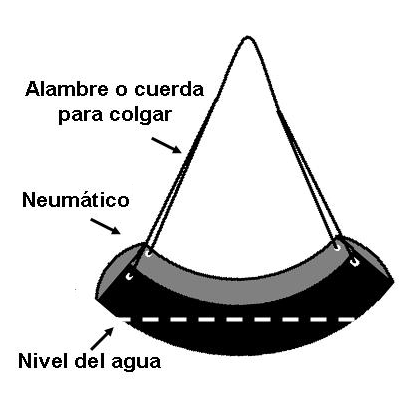
\includegraphics[width=\textwidth]{../book/anexos/graphics/disenho-1.png}

          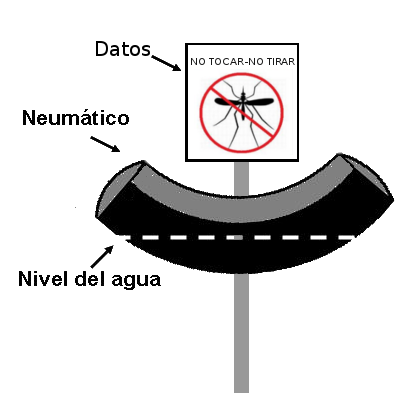
\includegraphics[width=\textwidth]{../book/anexos/graphics/disenho-2.png}
        \end{column}
        \begin{column}[c]{7cm}
          \begin{itemize}
            \item Criadero artificial y controlado.
            \item Se basan en la detección del vector en su etapa larval.
            \item Brinda información sobre los patrones de actividad espacial y estacional de ovipostura.
            \item Permiten reconocer las condiciones climáticas favorables para la eclosión y desarrollo larvario.
            \item Materiales reciclados como materia prima.
          \end{itemize}
        \end{column}
      \end{columns}
  \end{center}
\end{frame}

\begin{frame}[t]{Motivación y Definición del Problema.\\\textit{Larvitrampas.}}
  \begin{center}
    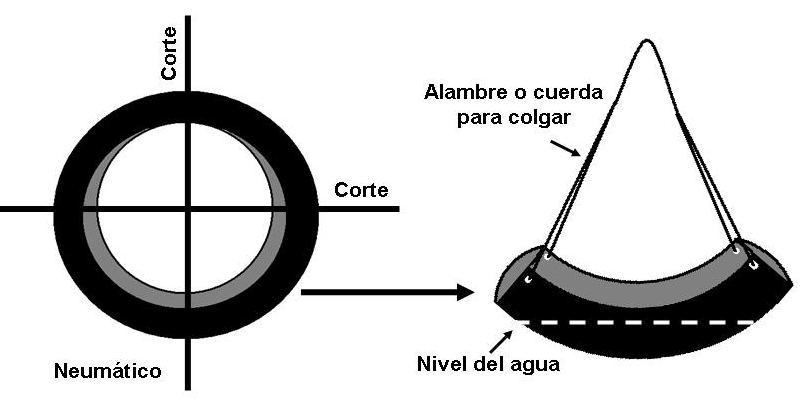
\includegraphics[width=9cm]{../book/anexos/graphics/construccion-larvitrampa.png}
  \end{center}
\end{frame}

%----------------------------6----------------------------------
\begin{frame}[t]{Motivación y Definición del Problema.\\\textit{La problemática del dengue en Paraguay.}}
  \begin{itemize}

    \item Las autoridades sanitarias del Paraguay no cuentan con datos computables, geográficamente, referentes al dengue, que permitan realizar análisis estadísticos y espaciales.

    \item Se deben diseñar y desarrollar herramientas para la recolección de la información, para su posterior análisis.

    \item Se deben optar por nuevas metodologías que permitan generar información para el análisis sin la necesidad de grandes requerimientos.

    \item Las larvitrampas y ovitrampas permiten generar información regionalizada sobre el estado y la distribución de la población del vector.

  \end{itemize}
\end{frame}


%--------------------------1------------------------------------
\begin{frame}[c]{Propuesta}
    \begin{center}
    Modelar y construir una herramienta que permita realizar estudios epidemiológicos de forma
    cartográfica, especializada para el particular caso del dengue, mediante la simulación de
    comportamiento del Aedes aegypti sometido a las variaciones climáticas correspondientes a la
    región con el fin de identificar focos de infestación.
    \end{center}
\end{frame}

%--------------------------2------------------------------------

\begin{frame}[c]{Objetivo General}
    \begin{center}
    Diseñar un modelo que permita analizar la extensión del vector del dengue y estudiar su posible
    relación con un potencial foco de riesgo, de forma a realizar una predicción de posibles focos
    de riesgo.
    \end{center}
\end{frame}


%--------------------------3------------------------------------
\begin{frame}[t]{Objetivos Especificos}
    \begin{center}

        \begin{itemize}
        \item Analizar nuevos métodos de muestreo de la abundancia poblacional del vector, con el fin de apoyar la lucha preventiva contra la enfermedad.

        \item Generar información relevante que pueda ayudar a las autoridades pertinentes para toma de decisiones en la lucha contra el dengue.

        \item Diseñar el modelo de forma paramétrica, para que sea aplicable a cualquier región o área de estudio.

        \item Implementar, un sistema computacional mediante el cual se puedan procesar y presentar los resultados obtenidos, en un sistema de información geográfica.
        \end{itemize}
    \end{center}
\end{frame}

%!TEX root = ../tesis.tex
\section{Descripci\'on General}
\label{sec:solucion-general}


%----------------------1----------------------------------------
\begin{frame}[t]{Resultados y discusión.\\\textit{Entorno de pruebas.}}
\begin{itemize}
	\item Comparar las tasas de desarrollo obtenidas con los resultados obtenidos por expertos en laboratorio.
	\item Analizar el comportamiento de la disperción de la población.
    \item Los parámetros de configuración fueron tomados del material bibliográfico de apoyo.
    \item El periodo de simulación fue de 50 días, a temperatura constante.
    \item La dirección del viento seleccionada fue la suroeste.
    \item Se generaron aleatoriamente 1.146 larvas para 25 puntos de control.
    \end{itemize}
\end{frame}

\begin{frame}[t]{Resultados y discusión. \textit{Población inicial.}}
    \begin{center}
        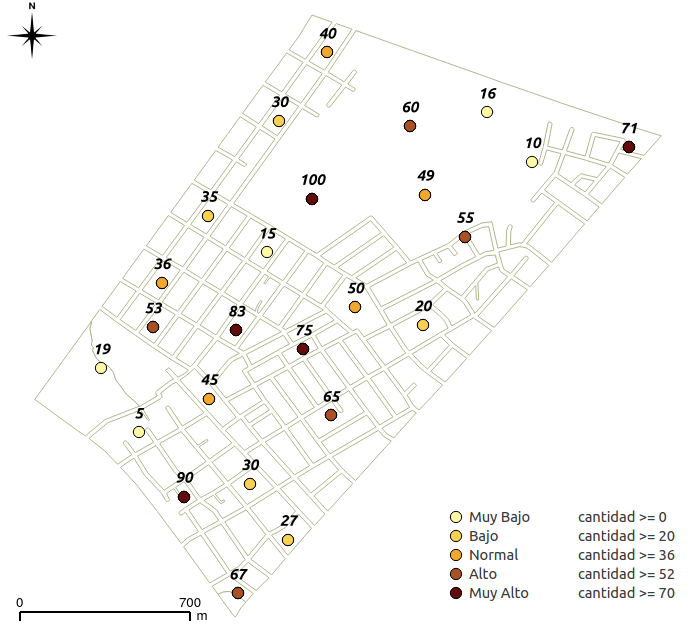
\includegraphics[width=7.5cm]{./graphics/extension-poblacion.png}
    \end{center}
\end{frame}
%--------------------------2------------------------------------
\begin{frame}[t]{Resultados y discusión.\\\textit{Tasas de desarrollo.}}
Los resultados obtenidos, fueron comparados con los valores observados por Beserra, Eduardo B. et al (2006) en : 
\\\text{}
\\\textit{Biologia e exigências térmicas de Aedes aegypti (L.) (Diptera: Culicidae) provenientes de quatro regiões bioclimáticas da Paraíba.}
\end{frame}

\begin{frame}[t]{Resultados y discusión.\\\textit{Tasas de desarrollo de los huevos.}}
    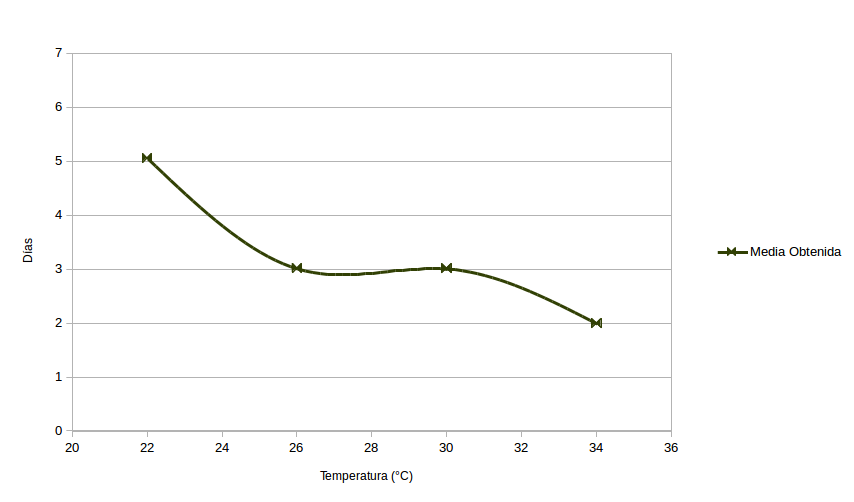
\includegraphics[width=\textwidth]{./graphics/huevos-desarrollo-single.png}
\end{frame}

\begin{frame}[t]{Resultados y discusión.\\\textit{Tasas de desarrollo de los huevos.}}
    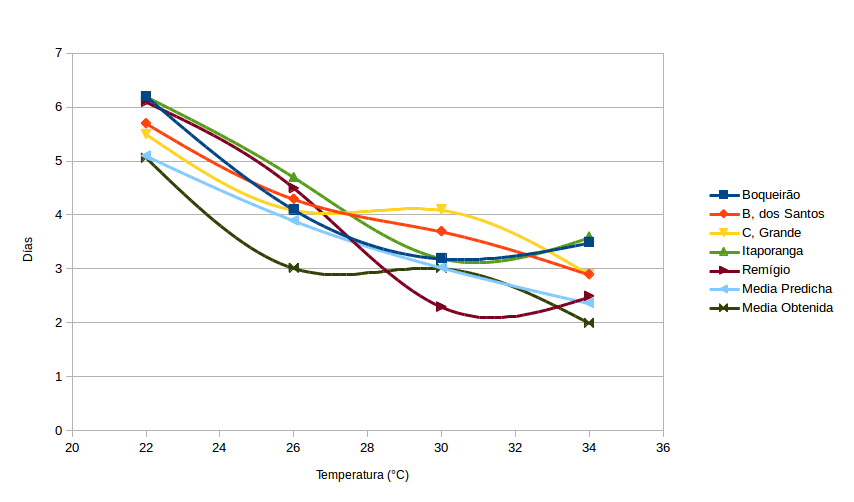
\includegraphics[width=\textwidth]{./graphics/huevos-desarrollo.png}
\end{frame}

\begin{frame}[t]{Resultados y discusión.\\\textit{Tasas de desarrollo de las larvas.}}
    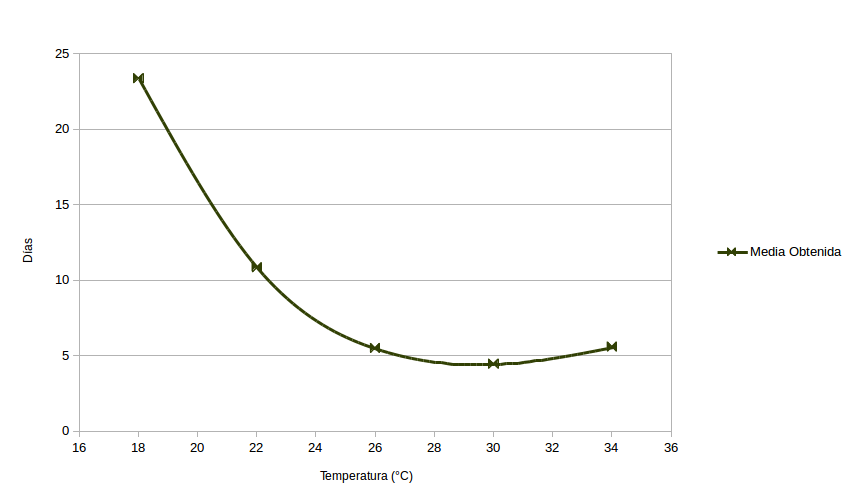
\includegraphics[width=\textwidth]{./graphics/larvas-desarrollo-single.png}
\end{frame}

\begin{frame}[t]{Resultados y discusión.\\\textit{Tasas de desarrollo de las larvas.}}
    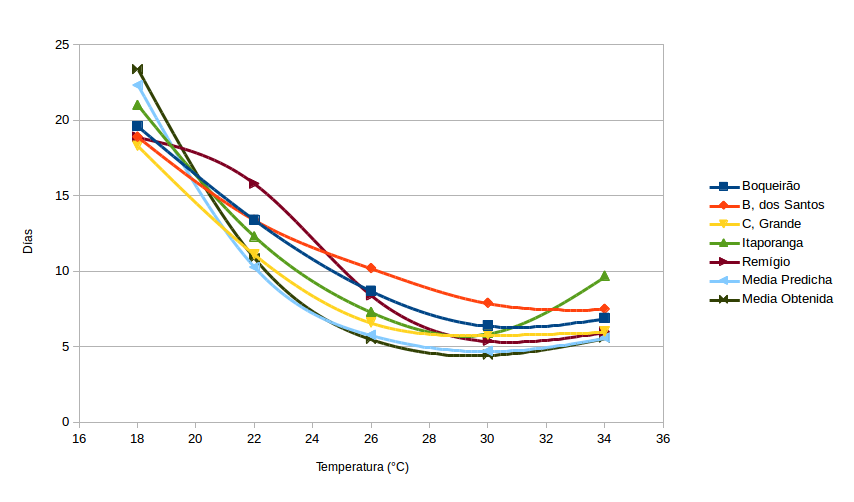
\includegraphics[width=\textwidth]{./graphics/larvas-desarrollo.png}
\end{frame}

\begin{frame}[c]{Resultados y discusión.\\\textit{Tasas de desarrollo de las pupas.}}
    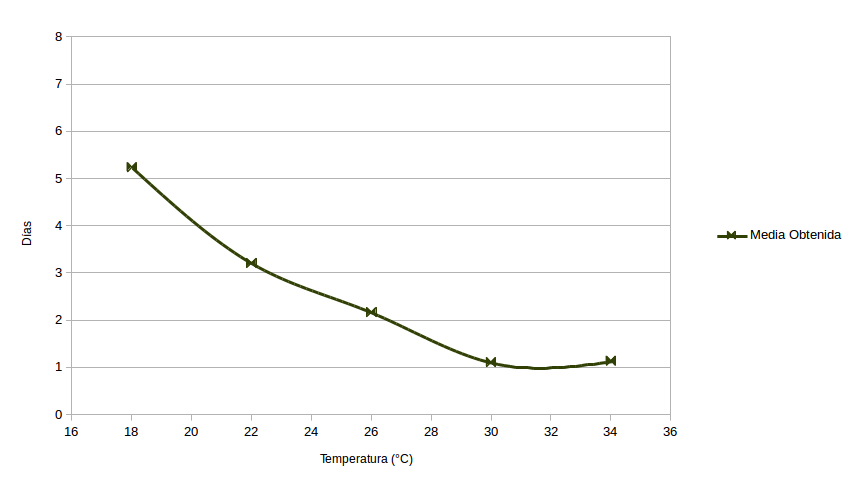
\includegraphics[width=\textwidth]{./graphics/pupas-desarrollo-single.png}
\end{frame}

\begin{frame}[c]{Resultados y discusión.\\\textit{Tasas de desarrollo de las pupas.}}
    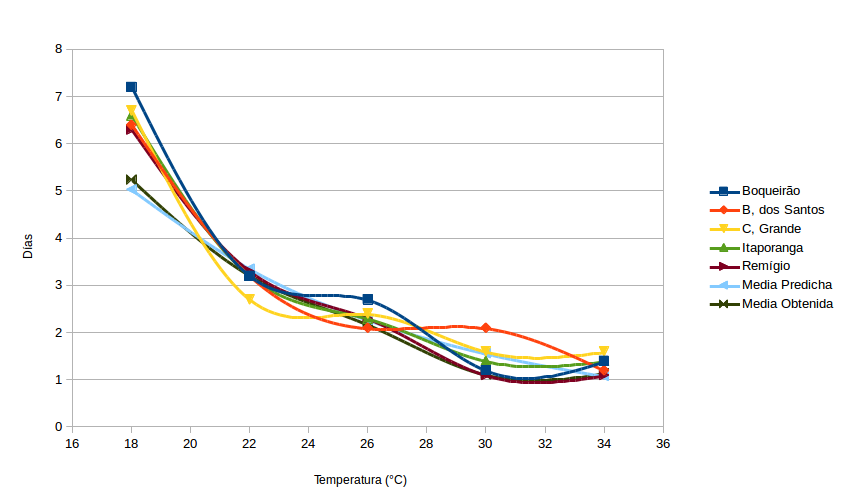
\includegraphics[width=\textwidth]{./graphics/pupas-desarrollo.png}
\end{frame}

\begin{frame}[t]{Resultados y discusión.\\\textit{Ciclo gonotrófico.}}
    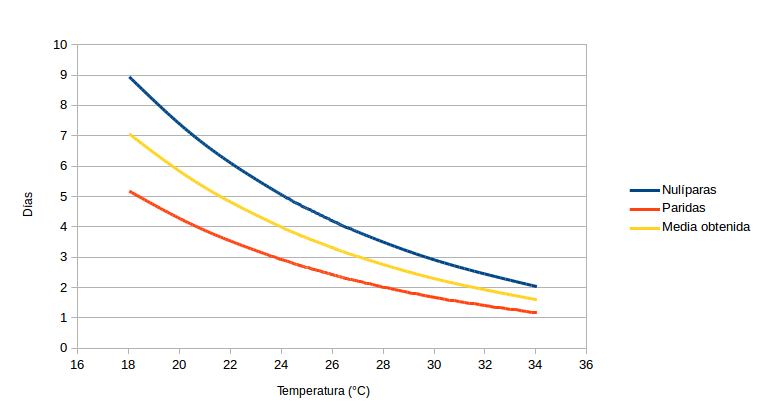
\includegraphics[width=\textwidth]{./graphics/ciclo-gonotrofico-temperatura.png}
\end{frame}

%--------------------------2------------------------------------

\begin{frame}[t]{Resultados y discusión.\\\textit{Crecimiento de la población en etapas inmaduras.}}
\begin{center}
    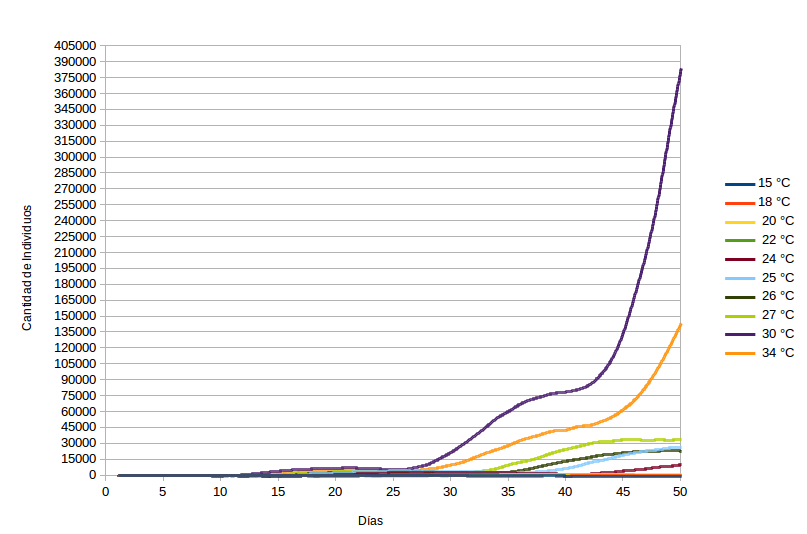
\includegraphics[width=9.3cm]{../paper/graphics/evolucion-poblacion-all.png}
\end{center}
\end{frame}

\begin{frame}[t]{Resultados y discusión.\\\textit{Crecimiento de la población en etapas inmaduras.}}
\begin{center}
\begin{figure}
     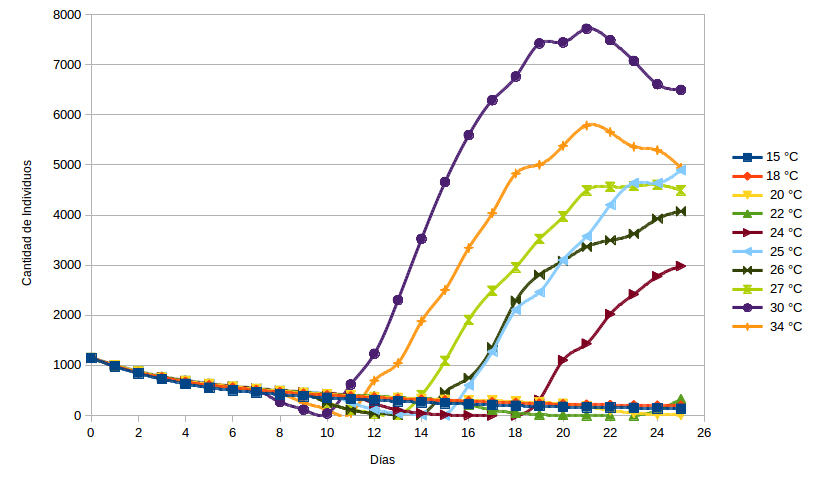
\includegraphics[width=9.3cm]{./graphics/poblacion-inmadura-p1.png}
     \caption{Del día 1 al 25.}
\end{figure}
\end{center}
\end{frame}

\begin{frame}[t]{Resultados y discusión.\\\textit{Crecimiento de la población en etapas inmaduras.}}
\begin{center}
\begin{figure}
    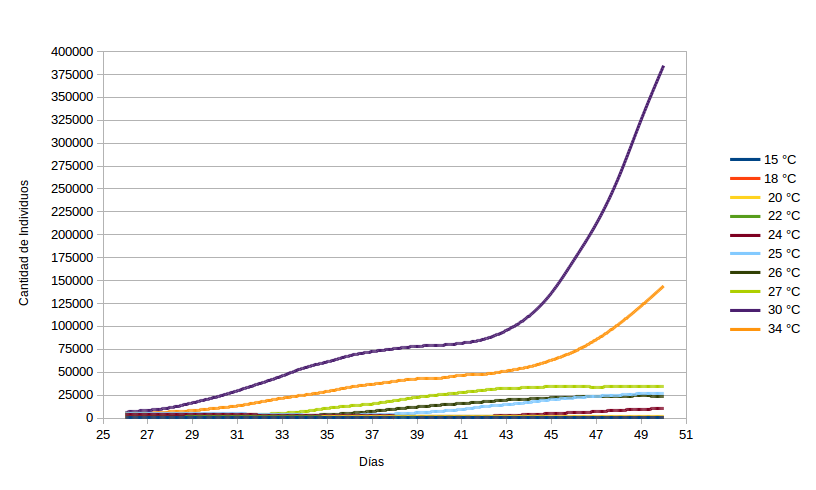
\includegraphics[width=9.3cm]{./graphics/poblacion-inmadura-p2.png}
    \caption{Del día 26 al 50.}
\end{figure}
\end{center}
\end{frame}

\begin{frame}[t]{Resultados y discusión.\\\textit{Crecimiento de la población de hembras adultas.}}
\begin{center}
    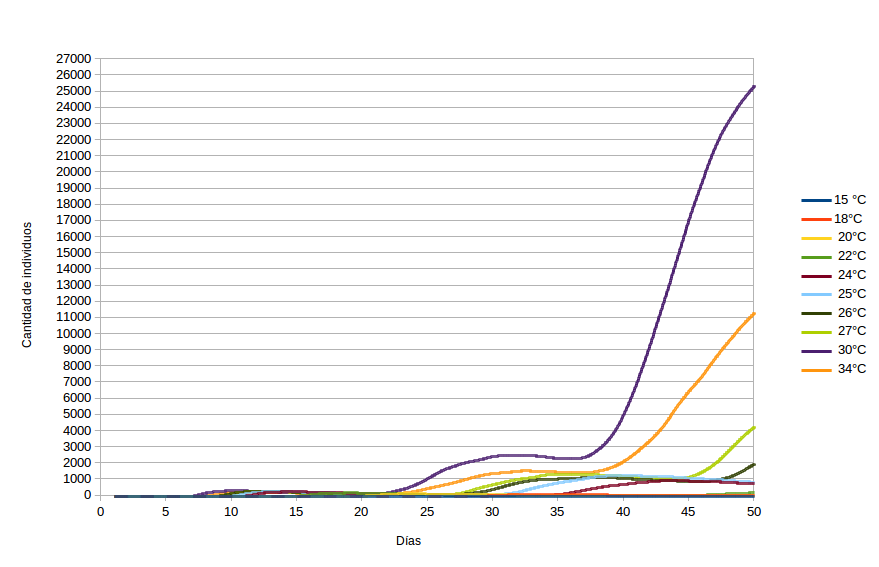
\includegraphics[width=9.3cm]{../paper/graphics/evolucion-poblacion-adultos.png}
\end{center}
\end{frame}

\begin{frame}[t]{Resultados y discusión.\\\textit{Crecimiento de la población de hembras adultas.}}
\begin{center}
\begin{figure}
    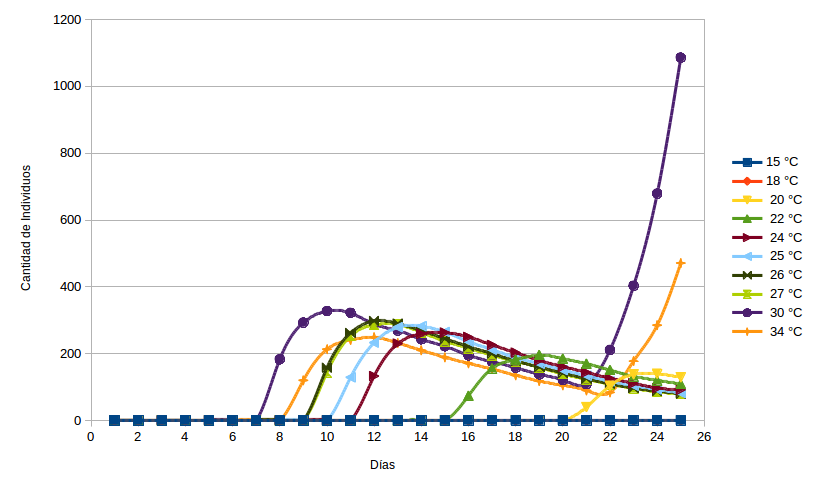
\includegraphics[width=9.3cm]{./graphics/poblacion-adulto-p1.png}
    \caption{Del día 1 al 25.}
\end{figure}
\end{center}
\end{frame}

\begin{frame}[t]{Resultados y discusión.\\\textit{Crecimiento de la población de hembras adultas.}}
\begin{figure}
    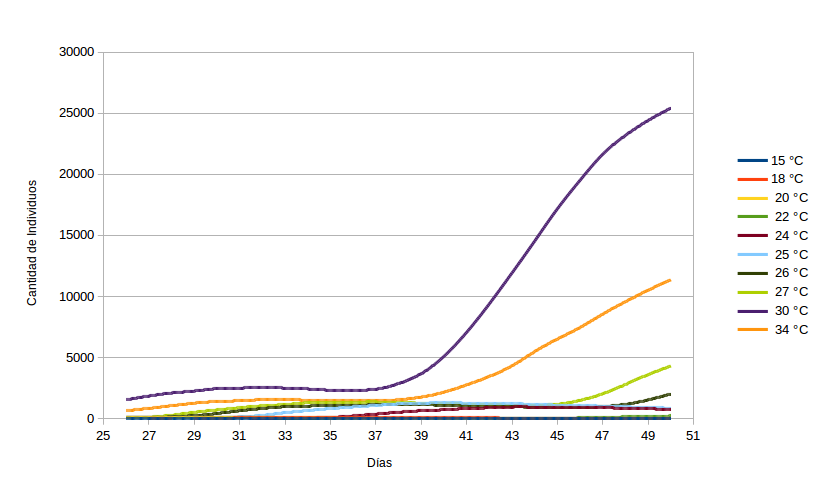
\includegraphics[width=9.3cm]{./graphics/poblacion-adulto-p2.png}
    \caption{Del día 26 al 50.}
\end{figure}
\end{frame}



\begin{frame}[t]{Resultados y discusión.\\\textit{Focos de infestación.}}
\begin{center}
    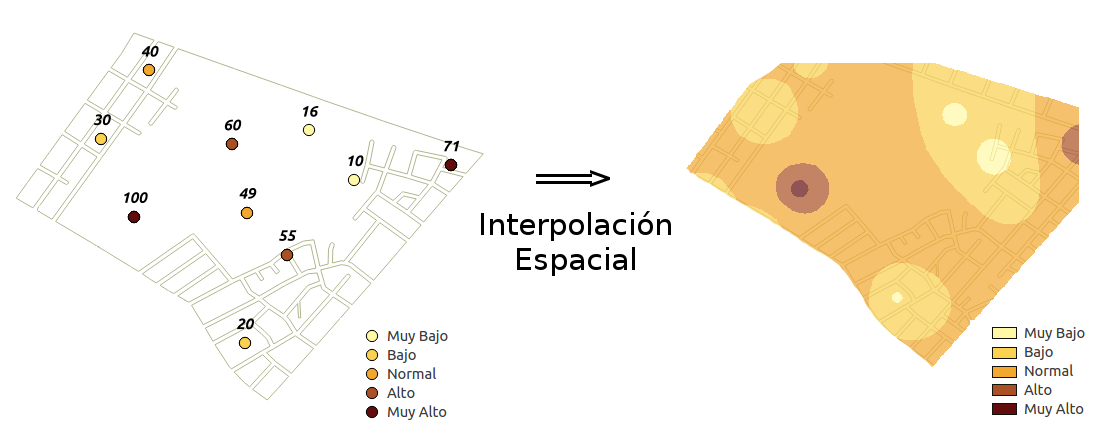
\includegraphics[width=11cm]{./graphics/identificacion-focos.png}
\end{center}
\end{frame}

\begin{frame}[t]{Resultados y discusión.\\\textit{Focos de infestación.}}
\begin{center}
\begin{table}[!hptb]
    \begin{minipage}{\textwidth}
    \scriptsize
    \centering
    \caption{\label{tab:niveles-riesgo-zonas} Clasificación de los niveles de infestación de acuerdo al tipo de zona.}
    \begin{tabular}{l l c c c}
        \hline\\
         Niveles de infestación & Tipo de zona & Mínimo $u(x,y)$$^a$ & Máximo $u(x,y)$$^a$ \\
        \hline
        \hline
        Muy bajo & Pésima  & 0  & 19 \\
        Bajo     & Mala    & 20 & 35 \\
        Medio    & Regular & 36 & 51 \\
        Alto     & Buena   & 52 & 69 \\
        Muy Alto & Óptima  & 70 & --$^b$\\
    \end{tabular}
    \footnotetext[1]{\scriptsize Rango mínimo y máximo de $u(x,y)$ permitido para el tipo de zona.}
    \footnotetext[2]{\scriptsize No se estableció un límite superior para este nivel. }
    \end{minipage}
\end{table}
\end{center}
\end{frame}

%--------------------------2------------------------------------
\begin{frame}[t]{Resultados y discusión.\\\textit{Análisis espacial de la población.}}
\begin{itemize}
	\item Mapas de interpolación para la identificación del los focos de infestación.
	\item Cartografía de las hembras del vector.
\end{itemize}
\end{frame}

\begin{frame}[t]{Resultados y discusión.\\\textit{Mapas de interpolación a 30 \textcelsius.}}
    \begin{figure}
    \begin{subfigure}[b]{0.45\textwidth}
        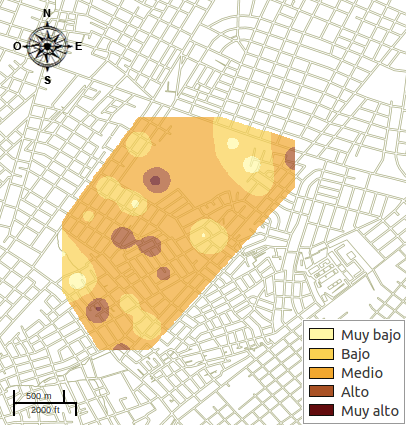
\includegraphics[width=\textwidth]{../book/capitulo-6/graphics/raster/temp-30-0.png}
        \caption{ Primer día de simulación.}
    \end{subfigure}
    ~~~~
    \begin{subfigure}[b]{0.45\textwidth}
        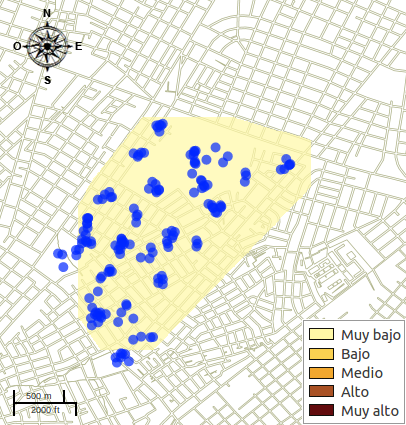
\includegraphics[width=\textwidth]{../book/capitulo-6/graphics/raster/temp-30-9.png}
        \caption{Día número 10 de simulación.}
    \end{subfigure}
    \end{figure}
\end{frame}


\begin{frame}[t]{Resultados y discusión.\\\textit{Mapas de interpolación a 30 \textcelsius.}}
    \begin{figure}
    \begin{subfigure}[b]{0.45\textwidth}
        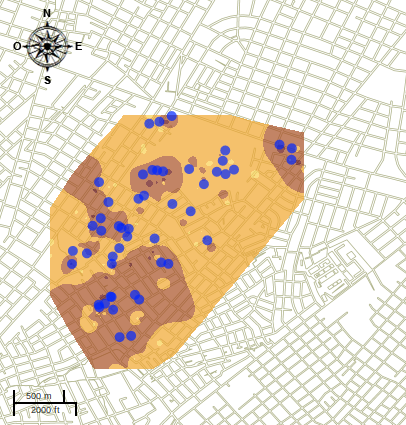
\includegraphics[width=\textwidth]{../book/capitulo-6/graphics/raster/temp-30-20.png}
        \caption{Día número 21 de simulación.}
    \end{subfigure}
    ~~~~
    \begin{subfigure}[b]{0.45\textwidth}
        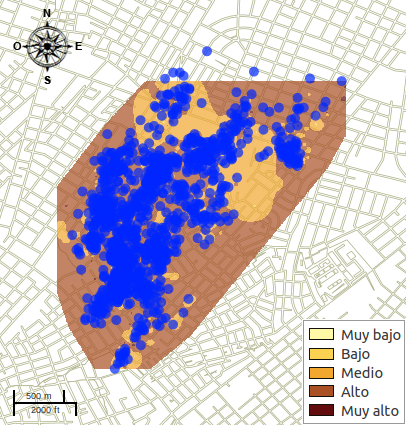
\includegraphics[width=\textwidth]{../book/capitulo-6/graphics/raster/temp-30-35.png}
        \caption{Día número 50 de simulación.}
    \end{subfigure}
    \end{figure}
\end{frame}

\section{Conclusión}
%(1) Diseñar un modelo que permita analizar la extensión del vector del dengue y estudiar su posible relación con un potencial foco de riesgo, de forma a realizar una predicción de posibles focos de riesgo.
En este trabajo presentó el diseño e implementación de un modelo predictivo para identificar focos
de infestación del, Aedes aegypti principal vector del dengue, sustentado en métodos de muestreo
para la determinación de la abundancia poblacional, modelos matemáticos para simular el ciclo de
vida del vector en un sistema de información geográfica, con el fin de apoyar a la lucha
preventiva de esta enfermedad. Para el diseño y desarrollo del simulador del proceso evolutivo, se
realizaron ciertas consideraciones que requieren la validación y revisión por parte de expertos en
el área, de forma que se puedan realizar los ajustes correspondientes para su aplicabilidad.El diseño e implementación del modelo como un simulador del proceso evolutivo del vector en el contexto de un sistema de información geográfica, permite realizaranálisis complejos de la realidad espacial rápidamente, generando información regionalizada para determinar los niveles de infestación correspondientes al área de estudio. Se considera al modelo resultante como genérico, debido a que sus parámetros pueden ser ajustados para aplicarlos en cualquier región o área de estudio, y extensible, teniendo en cuenta que puede ser modificado para incluir nuevas variables y procesos.

%(3)Diseñar el modelo de forma paramétrica y escalable, para que sea aplicable y extensible a cualquier región o área de estudio.
El simulador de proceso evolutivo se encuentra compuesto por modelos, ampliamente respaldados por
el material bibliográfico, en \cite{sharpe1977reaction, focks1993dynamic, schoolfield1981non, otero2006stochastic, rueda1990temperature}, que son utilizados para el cálculo de las tasas de
desarrollo y mortalidad de las distintas etapas de desarrollo del ciclo de vida del vector. La
configuración del simulador del proceso evolutivo requiere de parámetros asociados con las
características biológicas y datos ecológicos correspondientes al área de estudio, por lo que para
su aplicación, estos parámetros de configuración deben ser validados por expertos en el área
mediante trabajos de campo. No obstante, utilizando valores tomados del material bibliográfico de
apoyo, se pudo observar un buen comportamiento de los resultados obtenidos mediante el simulador
del proceso evolutivo. Solo presentan pequeñas variaciones en comparación con los valores
observados por expertos en laboratorio en condiciones controladas. Las variaciones observadas
pueden ser causadas por los distintos rasgos característicos de las cepas de mosquitos, utilizadas
en los estudios de referencia, que permiten una mayor o menor tolerancia a ciertas condiciones.

%(4)Generar información relevante que pueda ayudar a las autoridades pertinentes para toma de decisiones en la lucha contra el dengue.
En un futuro, con los ajustes y validaciones correspondientes a ser realizadas por expertos en el
área, la información generada por el simulador del proceso evolutivo del Aedes aegypti, asociada
con niveles de infestación y los mapas de interpolación podrían, permitir a las autoridades
sanitarias, del Paraguay, definir y planificar, de forma más efectiva, las medidas de control,
prevención y logística a realizar con con el fin de disminuir los niveles de infestación en una
región.


%----------------------1----------------------------------------
\begin{frame}[t]{Trabajos futuros}
    \begin{center}
        \begin{itemize}
            \item Incluir otras variables con el fin de analizar su relación y el impacto de las mismas con las zonas de riesgo.

            \item Impacto de las lluvias en la generación de sitios de reproducción.

            \item Tener en cuenta las limitaciones geográficas a la hora del vuelo y la ovipostura.

            \item Optimizacíon de las rutas de fumigación y analizar el efecto de la fumigación en el desarrollo de ciclo de vida del vector.

            \item Paralelizar el simulador del proceso evolutivo para optimizar el tiempo de respuesta y distribuir mejor las tareas de procesamiento.

            \item Analizar otros métodos de PDI con el fin de mejorar la confianza y la precisión de conteo de larvas.
        \end{itemize}
    \end{center}
\end{frame}

%----------------------1----------------------------------------
\begin{frame}[t]{Aportes}
    \begin{itemize}
        \item Escala de clasificación de niveles de infestación.
        \item Conteo de larvas mediante el proceso digital de imágenes.
        \item Un modelo y una herramienta genérica aplicable a cualquier área de estudio.
        \item Un simulador del proceso evolutivo del vector.
        \item Una herramienta web para la adminstación y análisis de los resultados.
        \item Generar inforamción que permita a las autoridades sanitarias a mejorar la plaficiación y lucha contra el dengue.
    \end{itemize}
\end{frame}

%----------------------1----------------------------------------
\begin{frame}{}
    \begin{center}
    Gracias por su atención.
    \end{center}
\end{frame}


%----------------------1----------------------------------------
\begin{frame}[c,plain]{}
    \begin{center}
    Anexos.
    \end{center}
\end{frame}

\begin{frame}[c]{Ovitrampas.}
  \begin{center}
    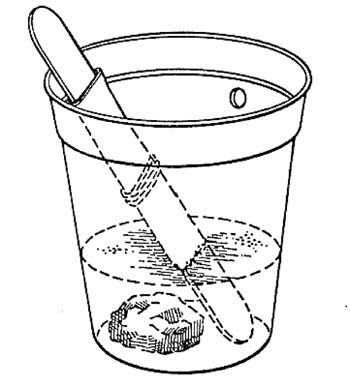
\includegraphics[width=6cm]{../book/capitulo-3/graphics/ovitrampa.jpg}
  \end{center}
\end{frame}

\begin{frame}[c]{Strack tecnológico.}
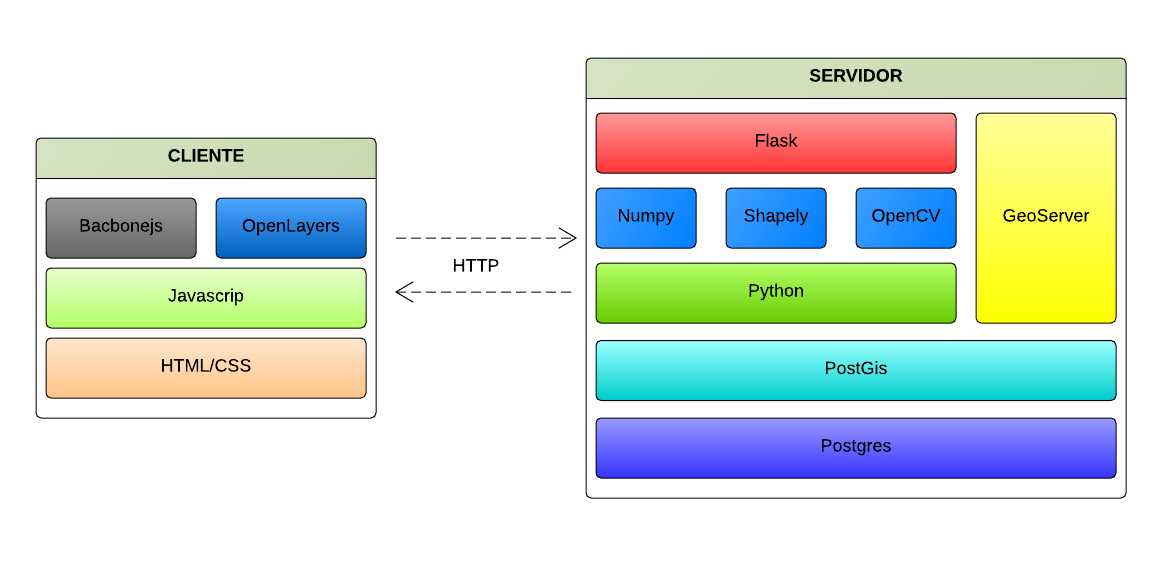
\includegraphics[width=\textwidth]{../book/capitulo-5/graphics/stack-tecnologias.png}
\end{frame}


\begin{frame}[c]{Conteo de larvas con PDI.}
    \begin{figure}
    \begin{subfigure}[b]{0.45\textwidth}
        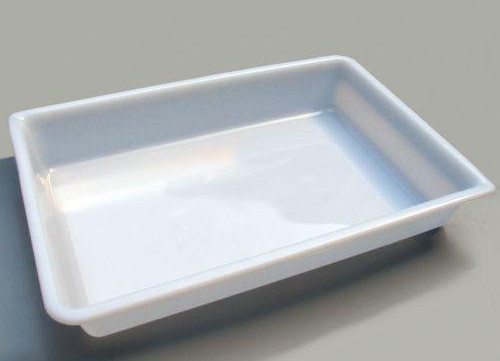
\includegraphics[width=4.5cm]{../book/capitulo-5/graphics/bandeja-muestra.jpg}
        \caption{Bandeja vacía.}
    \end{subfigure}
    ~~~~
    \begin{subfigure}[b]{0.45\textwidth}
        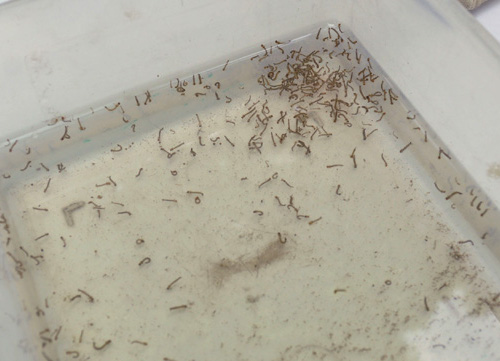
\includegraphics[width=4.5cm]{../book/capitulo-5/graphics/larvas-dengue.jpg}
        \caption{Bandeja con larvas.}
    \end{subfigure}
    \end{figure}
\end{frame}

\begin{frame}[c]{Conteo de larvas con PDI (2).}
    \begin{figure}
    \begin{subfigure}[t]{0.45\textwidth}
        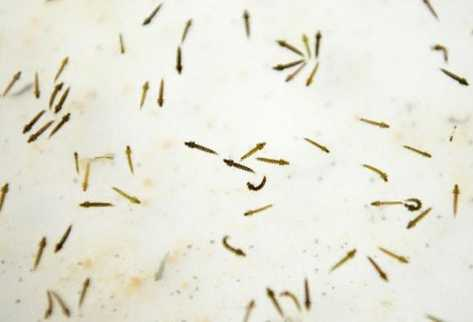
\includegraphics[width=4.5cm]{../book/capitulo-5/graphics/larvas-original.png}
        \caption{Imagen original.}
    \end{subfigure}
    ~~~~
    \begin{subfigure}[t]{0.45\textwidth}
        
\includegraphics[width=4.5cm]{../book/capitulo-5/graphics/larvas-otsu.png}
        \caption{Imagen luego de la umbralización.}
    \end{subfigure}
    \end{figure}
\end{frame}

\begin{frame}[t]{Coeficientes del modelo de Sharpe y DeMichele.}
\begin{table}
\begin{minipage}{\textwidth}
    \centering
    \small
    \caption{ \label{tab:coef-sharpe-demichele} Coeficientes para el modelo simplificado de Sharpe y DeMichele, con inhibición de altas temperaturas presentado por Schoolfield.}
    \begin{tabular}{l c r r r r }
        \hline \\
        Ciclo de desarrollo    & $R(298K)$ & $\Delta H_{A}$ & $\Delta H_{H}$ & $\Delta T_{1/2}$  \\
        \hline
        \hline
        Eclosión de los huevos$^a$ & 0,24000 & 10798,00 &  100000,00  & 14184,000\\
        Desarrollo larvario$^b$    & 0,20429 & 36072,78 &   59147,51  &   301,560\\
        Desarrollo pupal$^b$       & 0,74423 & 19246,42 &    5954,35  &   302,687\\
        Ciclo gonotrófico (AN)$^c$ & 0,21600 & 15725,00 & 1756481,00  &   447,200\\
        Ciclo gonotrófico (AP)$^c$ & 0,37200 & 15725,00 & 1756481,00  &   447,200\\
    \end{tabular}
    \footnotetext[1]{Coeficientes Otero et al., 2006.}
    \footnotetext[2]{Coeficientes Rueda et al.,1990.}
    \footnotetext[3]{Coeficientes, para AP y AN, tomados Otero et al., 2006.}
\end{minipage}
\end{table}
\end{frame}


\end{document}
